\section{Evaluation}\label{sec:eval}

\begin{table*}
  \centering
  \caption{The analysis precision of $\tool$ without refinement
  (\stextsf{no-refine}), with refinement (\stextsf{refine}), and their
  difference ($\Delta$)}
  \label{table:precision}
  \resizebox{\textwidth}{!}{%
    \begin{tabular}{c|l?r@{~}c@{~}r@{~}l@{}r|r@{~}c@{~}r@{~}l@{}r?r@{~}c@{~}r@{~}l@{}r|r@{~}c@{~}r@{~}l@{}r?r@{~}c@{~}r@{~}l@{}r|r@{~}c@{~}r@{~}l@{}r}
      \multirow{2}{*}{\textbf{Checker}} &
      \multirow{2}{*}{\textbf{Bug Kind}} &
      \multicolumn{30}{c}{
        \textbf{Precision = (\# True Bugs) / (\# Detected Bugs)}
      }\\\cline{3-32} &&
      \multicolumn{10}{c?}{\stextsf{\footnotesize no-refine}} &
      \multicolumn{10}{c?}{\stextsf{\footnotesize refine}} &
      \multicolumn{10}{c}{$\Delta$}\\

      \specialrule{.1em}{.0em}{.0em}

      \myrowc
      {\mr{2}{\stextsf{\scriptsize Reference}}}
      {\me{2}{60}{125}{48.0}} {\me{2}{61}{98}{62.2}} {\me{2}{+1}{-27}{+14.2}}
      {\mr{1}{\stextsf{\scriptsize UnknownVar}}}
      {\me{1}{17}{81}{21.0}} {\me{1}{17}{53}{32.1}} {\me{1}{}{-28}{+11.1}}

      \myrowh
      {\mr{1}{\stextsf{\scriptsize DuplicatedVar}}}
      {\me{1}{43}{44}{97.7}} {\me{1}{44}{45}{97.8}} {\me{1}{+1}{+1}{+0.1}}

      \hline

      \smyrowc
      {\mr{1}{\stextsf{\scriptsize Arity}}}
      {\mr{1}{\stextsf{\scriptsize MissingParam}}}
      {\me{1}{4}{4}{100.0}} {\me{1}{4}{4}{100.0}} {\me{1}{}{}{}}

      \hline

      \smyrowc
      {\mr{1}{\stextsf{\scriptsize Assertion}}}
      {\mr{1}{\stextsf{\scriptsize Assertion}}}
      {\me{1}{5}{57}{8.8}} {\me{1}{5}{31}{16.1}} {\me{1}{}{-26}{+7.4}}

      \hline

      \myrowc
      {\mr{2}{\stextsf{\scriptsize Operand}}}
      {\me{2}{22}{113}{19.5}} {\me{2}{22}{44}{50.0}} {\me{2}{}{-69}{+30.5}}
      {\mr{1}{\stextsf{\scriptsize NoNumber}}}
      {\me{1}{2}{65}{3.1}} {\me{1}{2}{6}{33.3}} {\me{1}{}{-59}{+30.3}}

      \myrowh
      {\mr{1}{\stextsf{\scriptsize Abrupt}}}
      {\me{1}{20}{48}{41.7}} {\me{1}{20}{38}{52.6}} {\me{1}{}{-10}{+11.0}}

      \specialrule{.1em}{.0em}{.0em}

      \mysrowh
      {\textbf{Total}}
      {91 / 299 (30.4\%)}{92 / 177 (52.0\%)}{+1 / -122 (+21.5\%)}

    \end{tabular}
  }
  \vspace*{-1.5em}
\end{table*}


We implemented $\tool$ as an open-source tool\footnote{The link is anonymized
because of a double-blind review process.} in Scala by extending $\jiset$, a
JavaScript IR-based semantics extraction toolchain~\cite{jiset}, with a worklist-based
fixpoint algorithm for type analysis. Thus, $\tool$ reports type-related specification bugs
detected in fully compiled abstract algorithms by $\jiset$.  For built-in libraries,
$\tool$ analyzes the abstract algorithms of the essential built-in objects: \jscode{Array},
\jscode{Object}, \jscode{Function}, \jscode{Math}, \jscode{Proxy}, and objects
for JavaScript primitive types.

We evaluate $\tool$ using the following research questions:
\begin{itemize}
  \item RQ1. \textbf{(Performance)} How long does $\tool$ take to perform type
    analysis for JavaScript specifications?
  \item RQ2. \textbf{(Precision)} How many type-related specification bugs
    detected by $\tool$ are true bugs?
  \item RQ3. \textbf{(Effectiveness of Refinement)} Does the condition-based refinement
    improve the analysis precision with modest performance overhead?
  \item RQ4: \textbf{(Detection of New Bugs)} Does $\tool$ detect new
    specification bugs in the latest version of ECMAScript?
\end{itemize}
Because the draft of the next ECMAScript (ES12, 2021) is fixed on March 9,
2021, we analyzed all 864 versions in the official
ECMAScript repository\footnote{https://github.com/tc39/ecma262} for the last
three years from January 1, 2018 to March 9, 2021.  We performed our experiments
on five Ubuntu machines equipped with 4.2GHz Quad-Core Intel Core i7 and 32GB of
RAM.


\subsection{Performance}\label{sec:performance}

Figure~\ref{fig:stat} shows the statistics of the type analysis using $\tool$ for
864 versions of ECMAScript: (a) the number of analyzed functions, (b) the number
of flow- and type-sensitive views, (c) the number of worklist iterations, and
(d) the analysis time.  For each version, $\tool$ analyzed
\inred{1,696.6} functions on average.  Since ECMAScript has gradually evolved,
it analyzed \inred{1,491} functions for the first version in 2018
but analyzed \inred{1,864} functions in the latest.
$\tool$ analyzes functions with flow- and type-sensitive views.
On average, each version has \inred{92.0}K views and each function has
\inred{54.1}~views.

We measured the performance of $\tool$ with the worklist iteration number
and the analysis time.  For each version of ECMAScript,
$\tool$ took \inred{137.3} seconds with \inred{301.6}K iterations of
the worklist algorithm on average.  The average analysis time consists of \inred{8.0} seconds
for the specification extraction (\stextsf{extract}),
\inred{128.5} seconds for the type analysis (\stextsf{analyze}), and
\inred{0.8} seconds for the bug detection (\stextsf{detect}).


\subsection{Precision}\label{sec:precision}

% \begin{table}
%   \centering
%   % 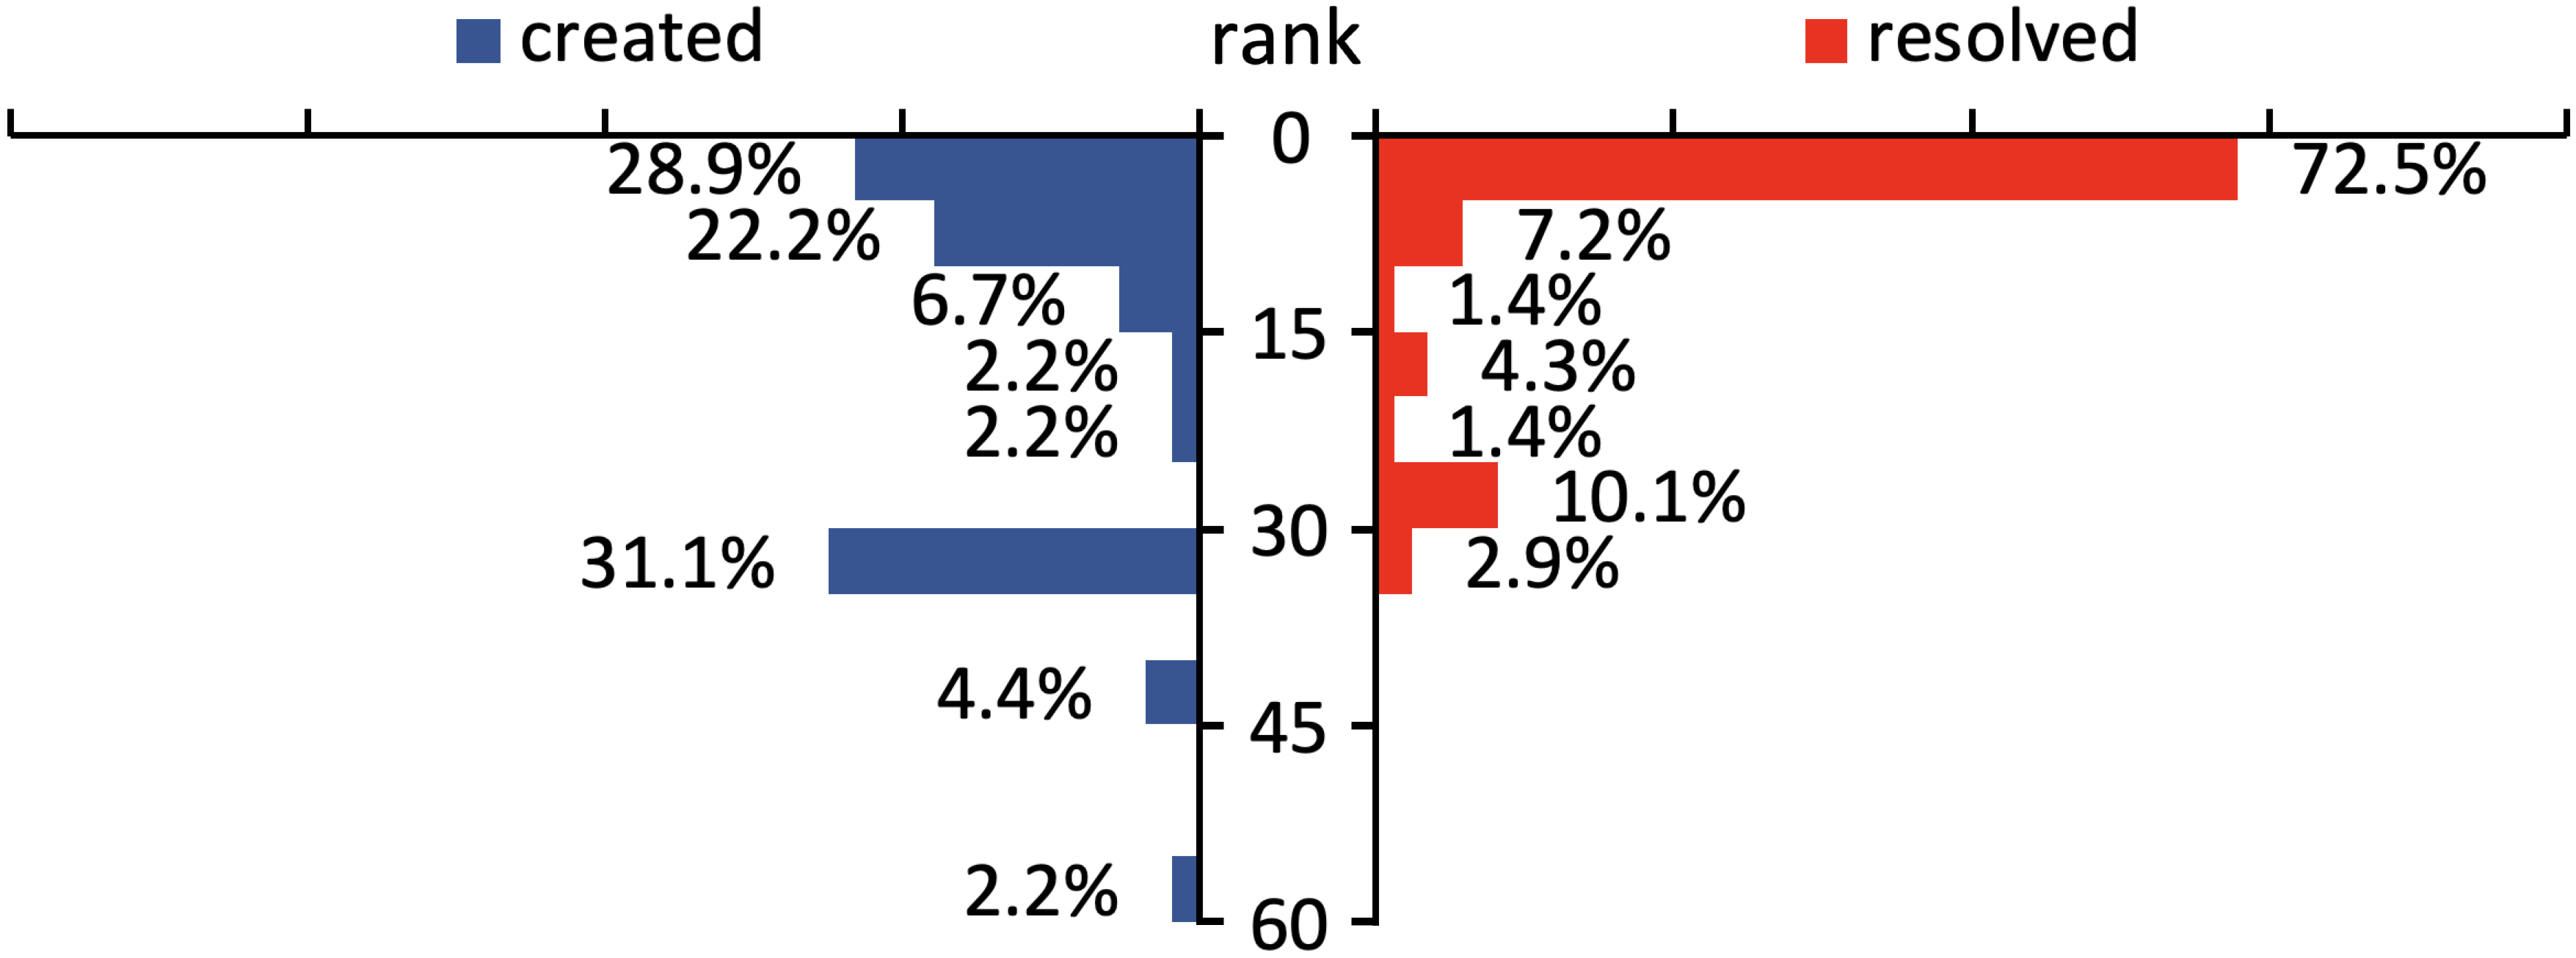
\includegraphics[width=\columnwidth]{img/author}
%   \caption{The creators and resolvers of true bugs.}
%   \label{fig:author}
%   \resizebox{\columnwidth}{!}{$
%     \inred{
%     \begin{array}{c?r|r|r|r|r|r?c?c}
%       \textbf{Rank} >
%       & 0 & 10 & 20 & 30 & 40 & 50
%       & \multicolumn{1}{c?}{\multirow{2}{*}{\textbf{Total}}}
%       & \multicolumn{1}{c}{\multirow{2}{*}{\textbf{Unknown}}}\\\cline{1-7}
%       \textbf{Rank} \leq
%       & 10 & 20 & 30 & 40 & 50 & 60
%       & & \\
% 
%       \specialrule{.1em}{.0em}{.0em}
% 
%       \textbf{\# Created}
%       & 23 & 4 & 1 & 14 & 2 & 1
%       & 45 & 46\\\hline
%       \textbf{\# Resolved}
%       & 57 & 6 & 12 & 2 & 0 & 0
%       & 77 & 14\\
% 
%     \end{array}
%     }
%   $}
%   \vspace*{-1em}
% \end{table}

\begin{figure}
  \centering
  \begin{subfigure}[b]{0.24\textwidth}
    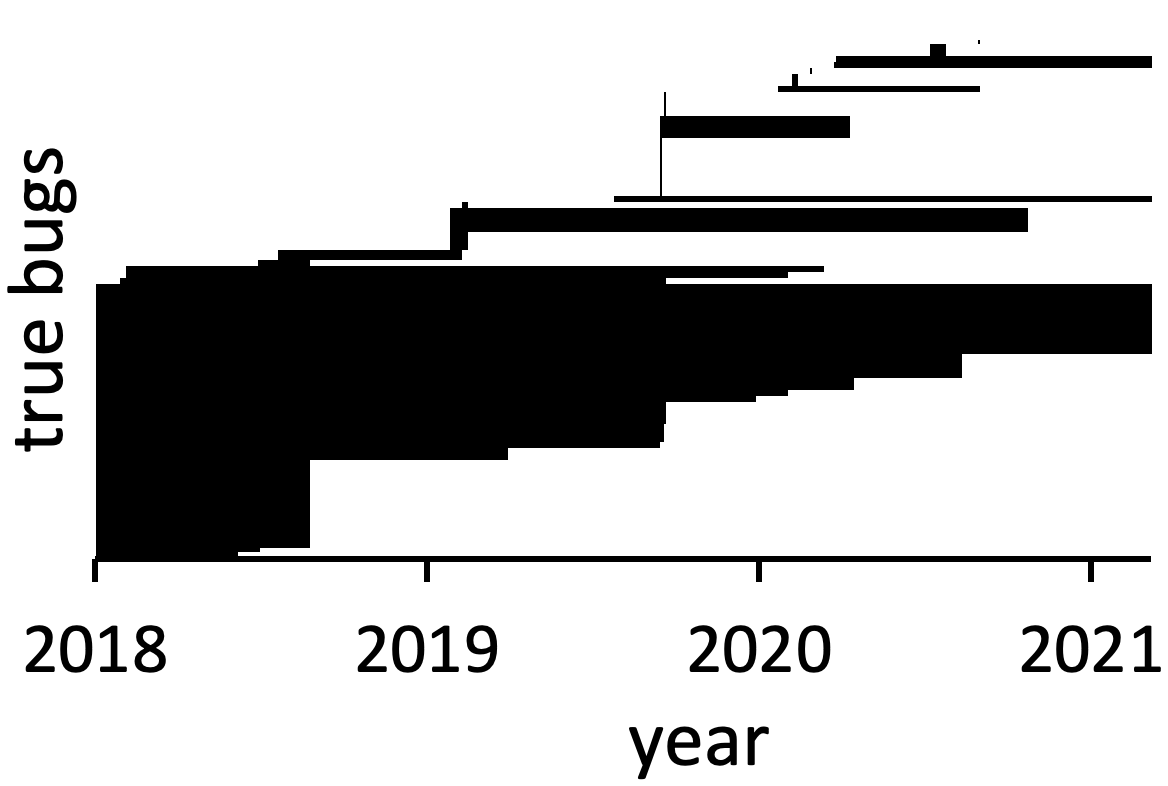
\includegraphics[width=\textwidth]{img/ttl-chro}
    \caption{TTLs sorted by creation time}
  \end{subfigure}
  \begin{subfigure}[b]{0.24\textwidth}
    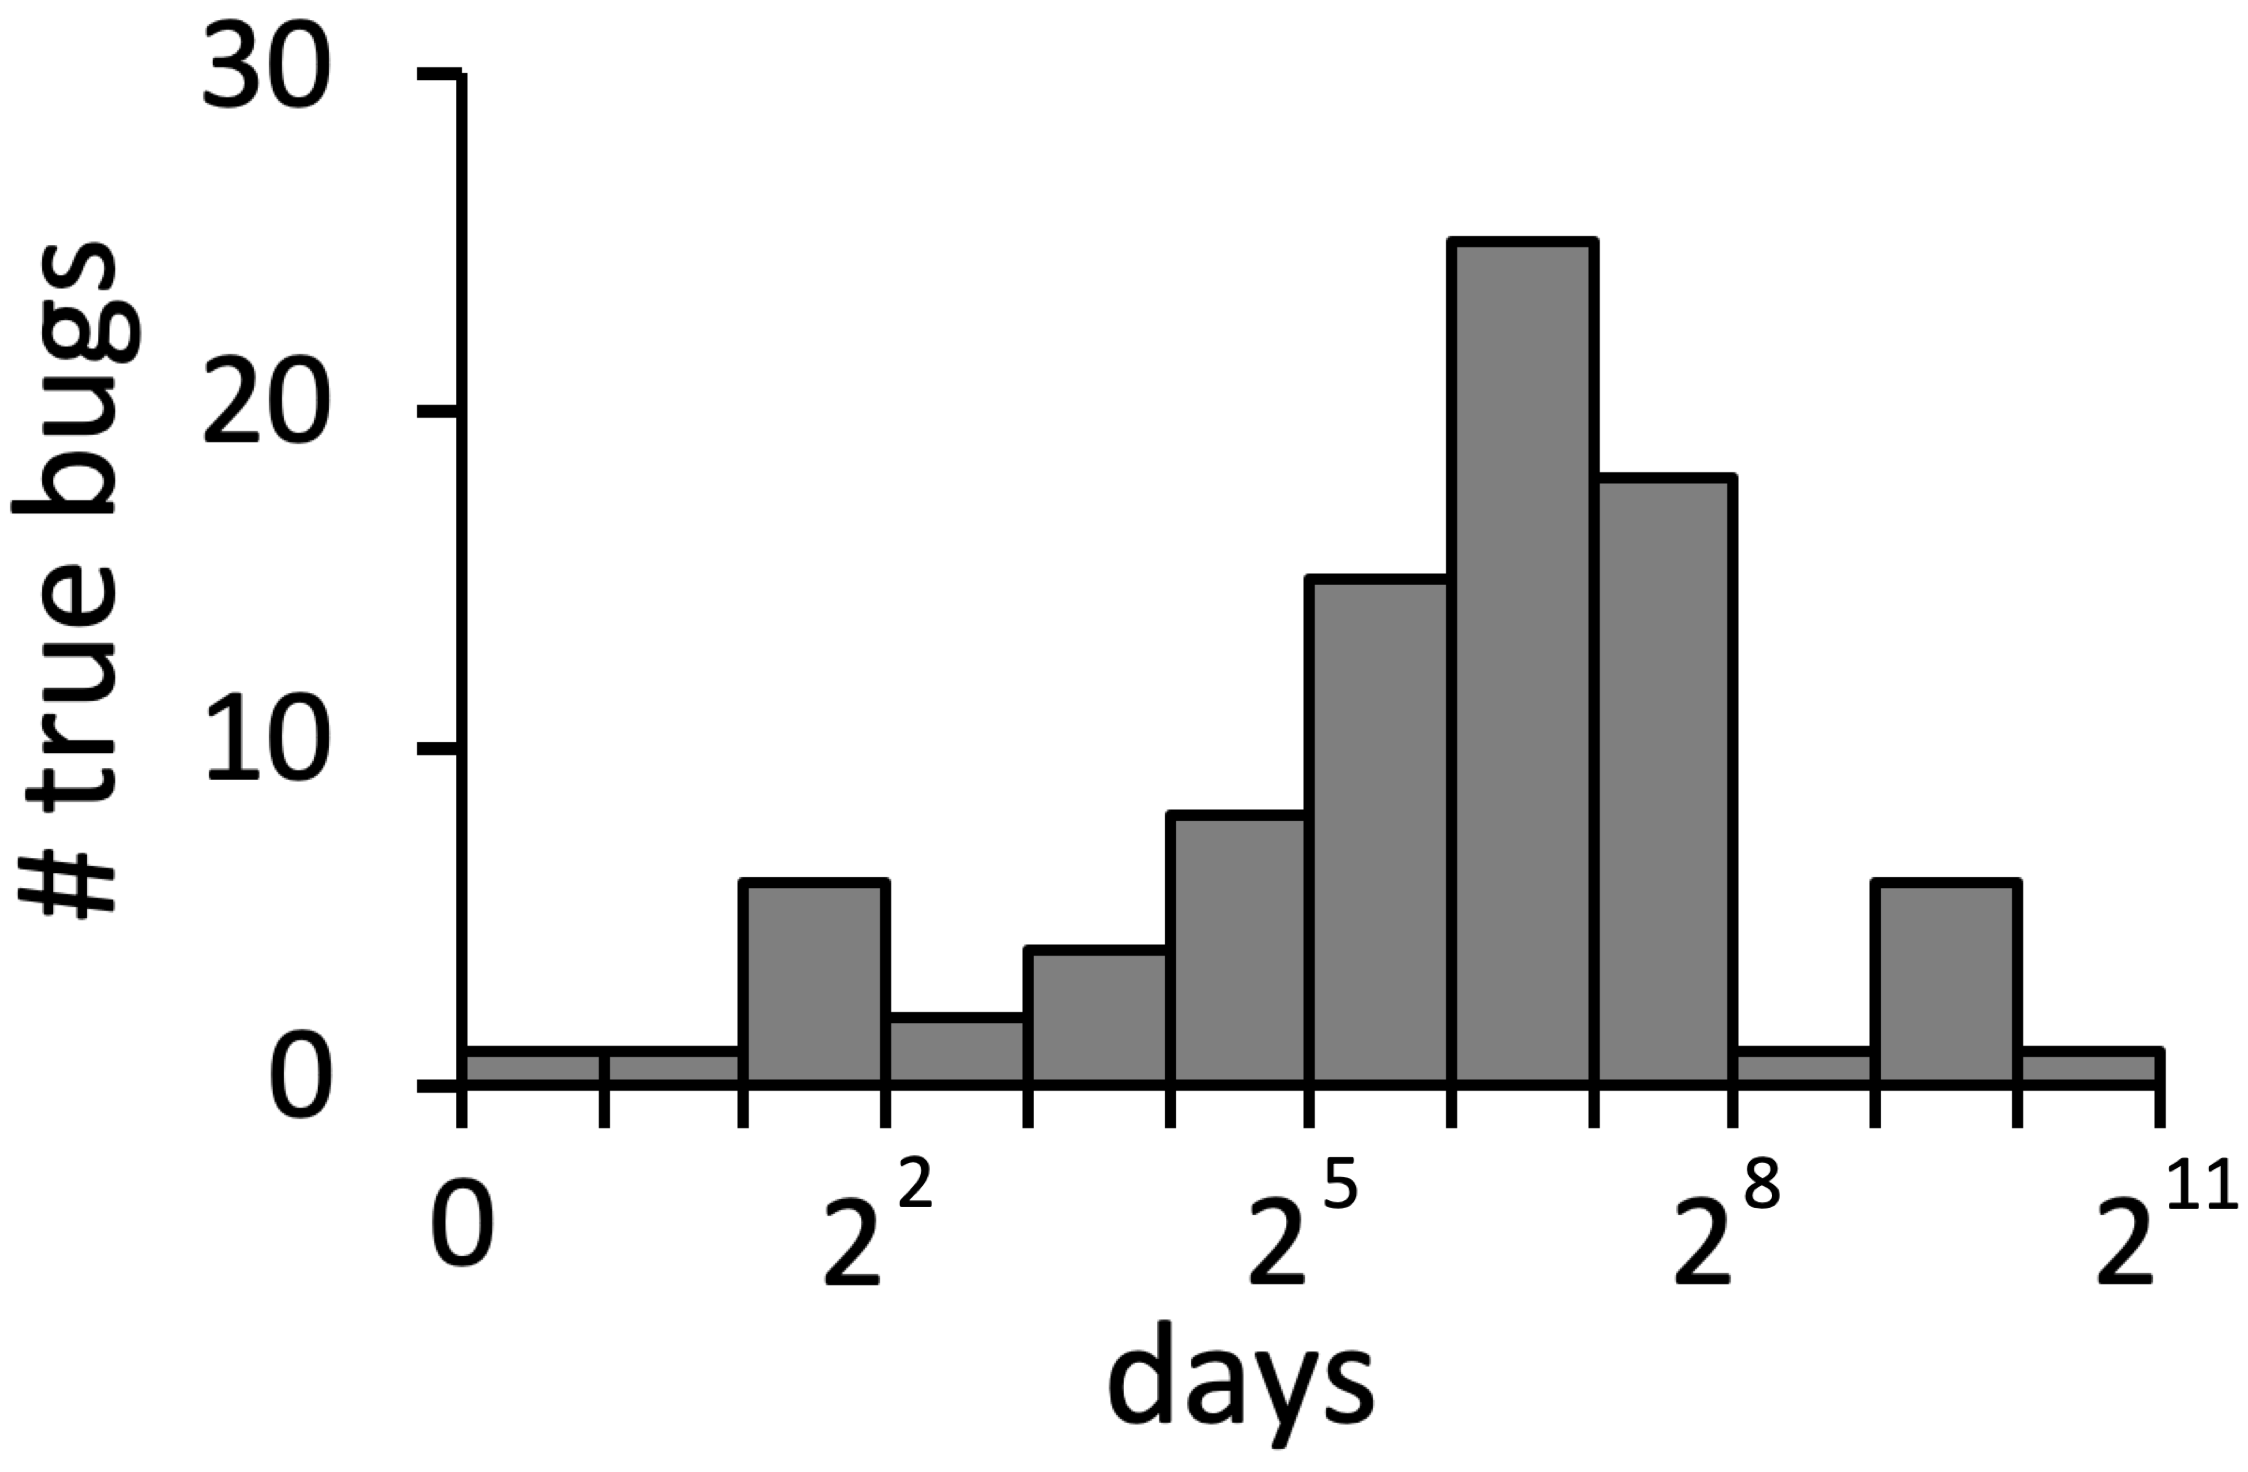
\includegraphics[width=\textwidth]{img/ttl-count}
    \caption{The histogram of TTLs}
  \end{subfigure}
  \caption{Time to Lives (TTLs) of true bugs}
  \vspace*{-1.5em}
  \label{fig:ttl}
\end{figure}

We measured the analysis precision with the number of true bugs in
the type-related specification bugs detected by $\tool$.
As summarized in the \stextsf{refine} column of Table~\ref{table:precision}, the analysis precision
is \inred{59.2}\%; \inred{93} out of \inred{157} detected bugs are true bugs.
The reference checker detected the most bugs with \inred{80.8}\% precision;
\inred{17} unknown variables (\stextsf{UnknownVar}) and
\inred{46} duplicated variable declarations (\stextsf{DuplicatedVar}) are true bugs.
We found \inred{four} missing parameters (\stextsf{MissingParam}) with \inred{100.0}\% precision and
\inred{four} assertion failures (\stextsf{Assertion}) with \inred{12.9}\% precision.
Finally, the operand checker detected
\inred{two} non-numeric operand bugs (\stextsf{NoNumber}) with \inred{33.3}\% precision and
\inred{20} unchecked abrupt completion bugs (\stextsf{Abrupt}) with \inred{52.6}\% precision.

To understand the severity of the detected true bugs, we extended $\tool$ to
automatically extract when they are created and resolved in the ECMAScript
official repository.  A bug is \textit{created} when it exists
in a specific version but does not exist in its previous version, and
a bug is \textit{resolved} vice versa. The \textit{Time to Live (TTL)} of a bug denotes
how many days the bug lasts.  Figure~\ref{fig:ttl} illustrates the TTLs of true bugs;
Figure~\ref{fig:ttl}(a) depicts the TTLs sorted by creation time and
Figure~\ref{fig:ttl}(b) depicts the histogram of the TTLs in a logarithmic scale.
Among \inred{93} true bugs, \inred{48} bugs are \textit{inherited},
which means that they are created before 2018,
and \inred{14} bugs still exist in the latest ECMAScript, which are newly detected by $\tool$.
We discuss the details of \inred{14} newly found bugs in Section~\ref{sec:new-bug}.
Even though we assume that \inred{48} inherited bugs are created on January 1, 2018,
the average TTL is \inred{414.5} and the maximum TTL is \inred{1,164}.
All the bugs with the maximum TTL are inherited ones and they are all newly detected.

We manually investigated \inred{64} false-positive bugs to understand why
$\tool$ detected them.  Among them, \inred{17} bugs are due to extraction failure
of mechanized specifications caused by wrong writing styles.
Because ECMAScript is written in HTML, $\jiset$ extracts abstract algorithms
using the \code{emu-alg} HTML tag.  Unfortunately, several abstract algorithms are
defined with the opening tag \code{<emu-alg>} but without the closing tag \code{</emu-alg>},
which causes extraction failure of mechanized specifications leading
to false-positive bugs.  The remaining \inred{47} bugs are due to imprecise analysis.
We found that \inred{28} bugs are due to imprecise analysis of the
conditions of assertions and branches for specific function calls.
For example, consider the following algorithm step for \textbf{GetValue}:
\begin{figure}[H]
  \centering
  \vspace*{-0.5em}
  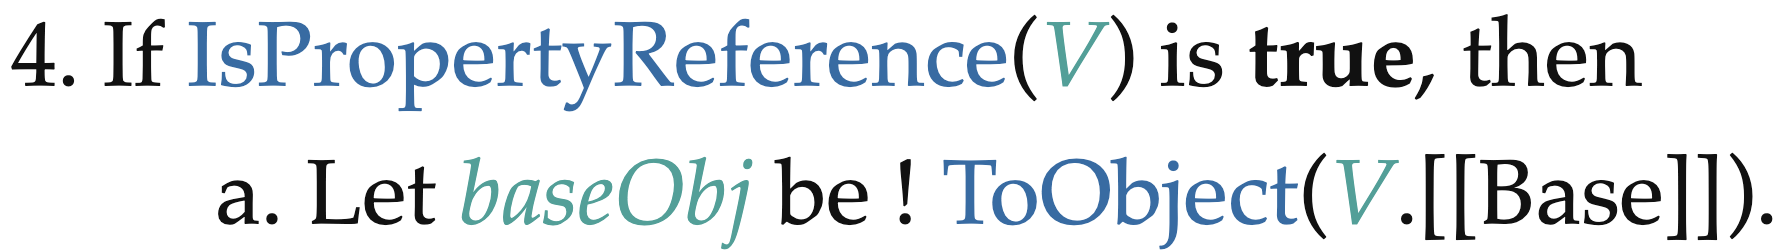
\includegraphics[width=0.7\columnwidth]{img/adv-refine-example}
  \vspace*{-0.5em}
\end{figure} \noindent
Since \textbf{IsPropertyReference} always returns
$\code{false}$ when the $\code{Base}$ field of a given reference record is
$\nconst{unresolvable}$, the field access $V$.[[Base]] cannot be
$\nconst{unresolvable}$ on line 4.a.  However, because the type analysis
does not compute such information,
$\nconst{unresolvable}$ is also passed as the argument of \textbf{ToObject}.
We believe that an advanced refinement technique can
resolve this problem by pruning out infeasible field types depending on specific contexts.


\begin{figure}
  \centering
  \begin{subfigure}[b]{0.24\textwidth}
    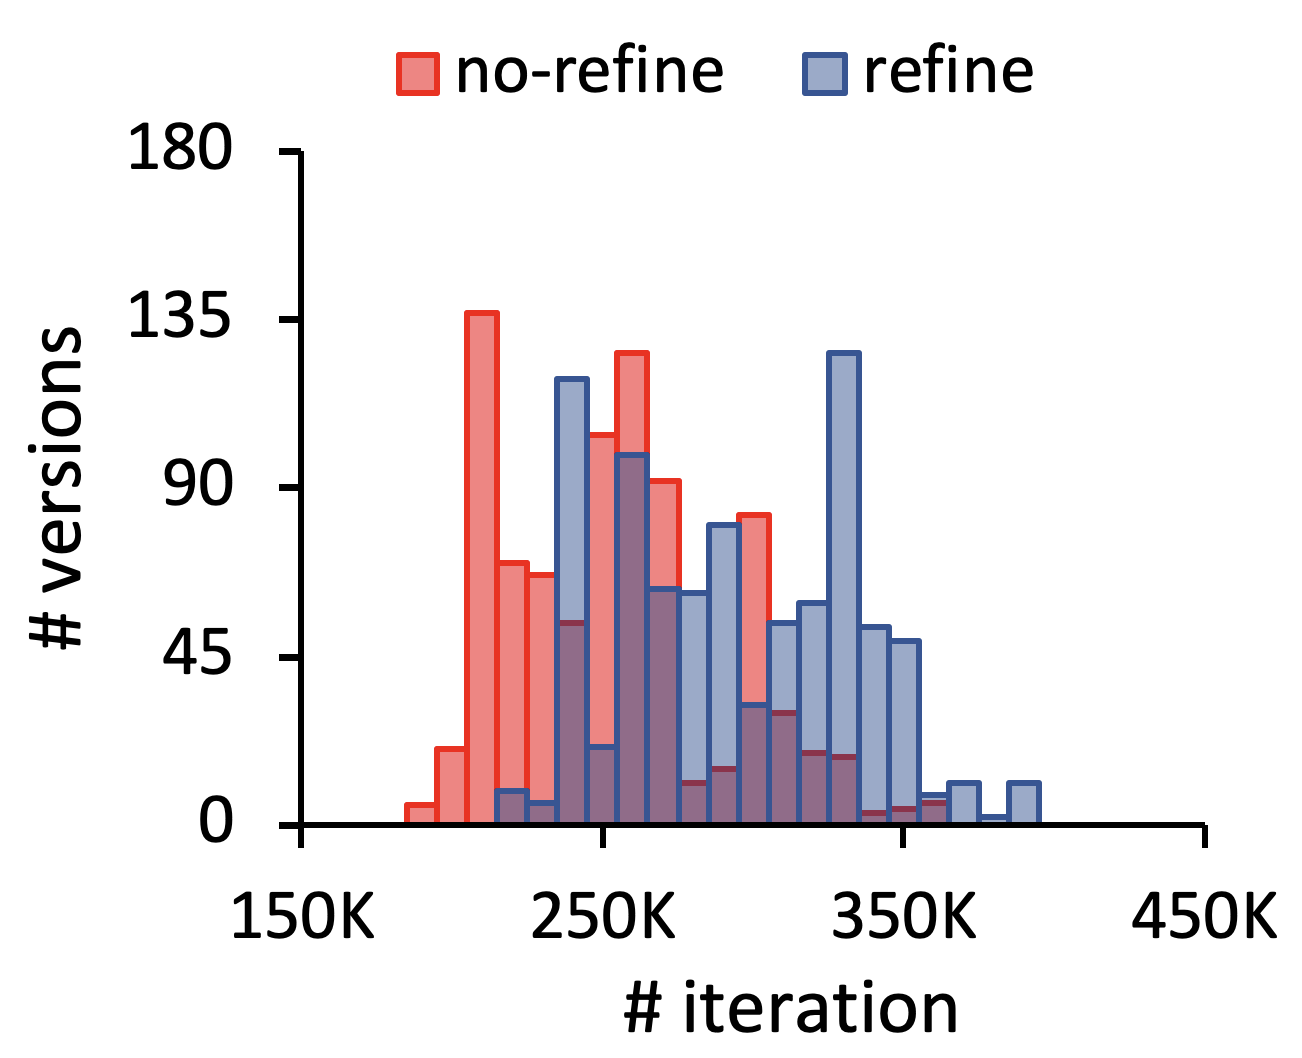
\includegraphics[width=\textwidth]{img/compare-iter}
    \caption{The histogram of iterations}
  \end{subfigure}
  \begin{subfigure}[b]{0.24\textwidth}
    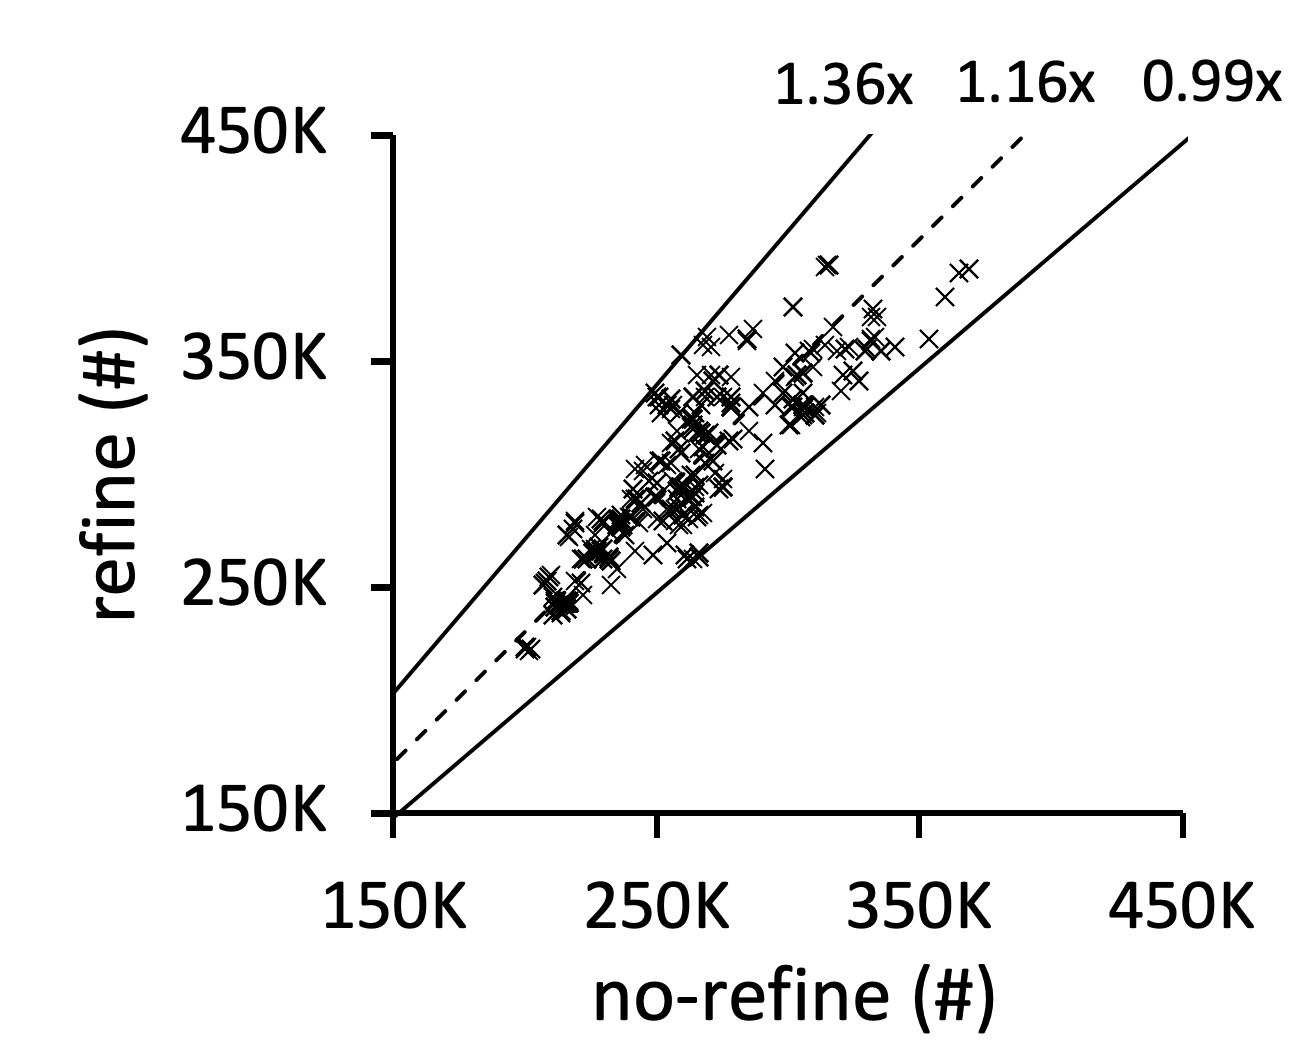
\includegraphics[width=\textwidth]{img/ratio-iter}
    \caption{The ratio of iterations}
  \end{subfigure}
  \begin{subfigure}[b]{0.24\textwidth}
    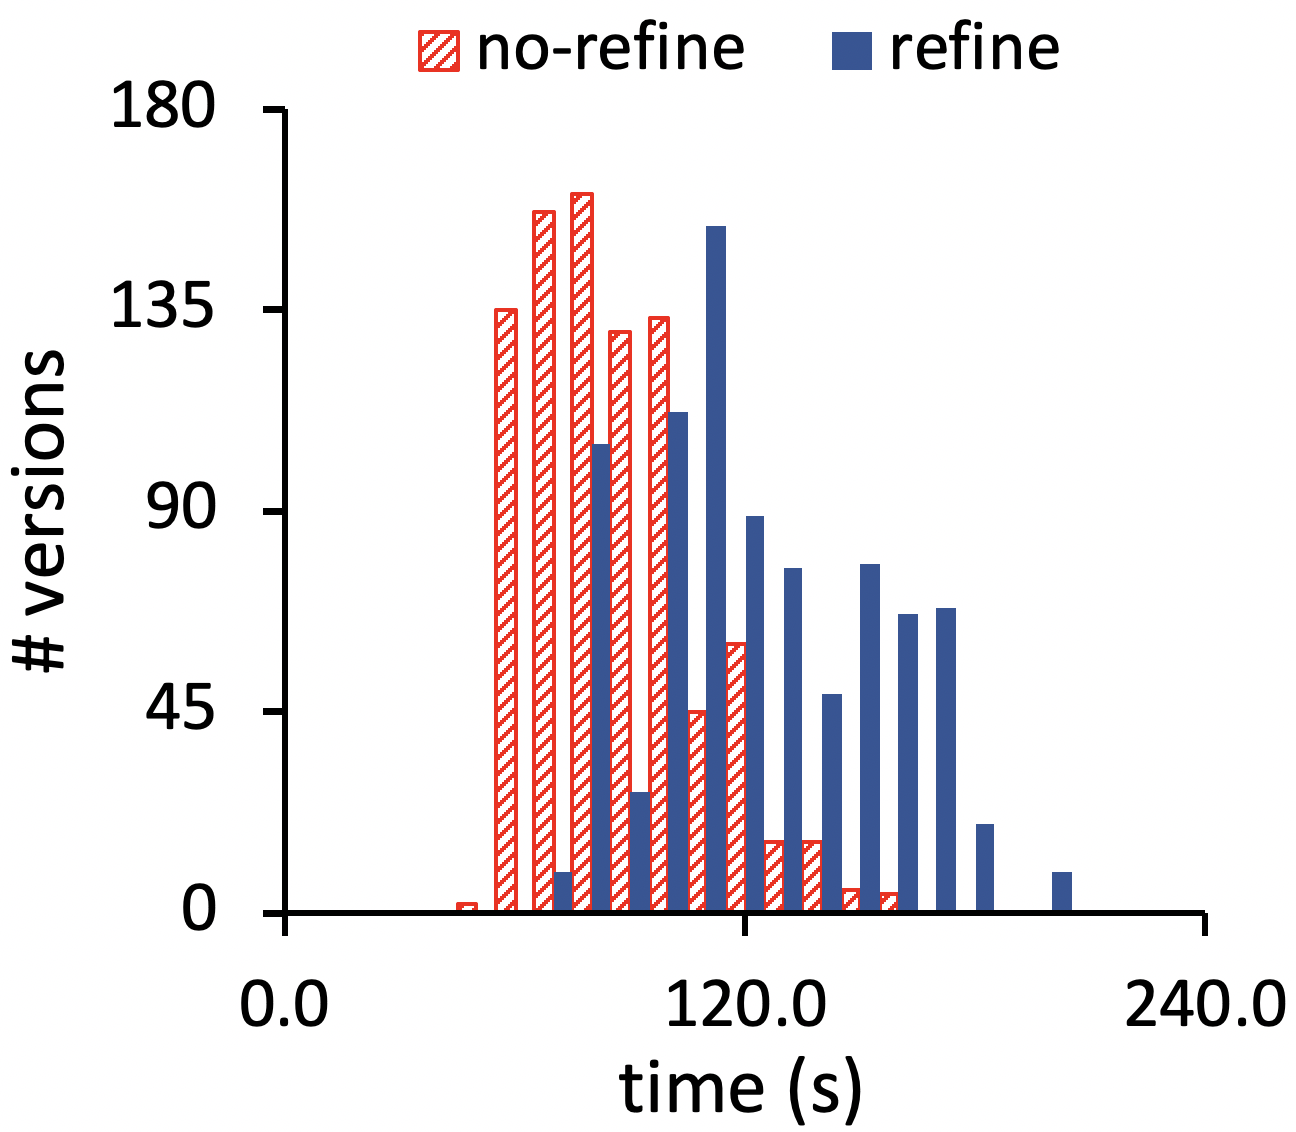
\includegraphics[width=\textwidth]{img/compare-time}
    \caption{The histogram of time}
  \end{subfigure}
  \begin{subfigure}[b]{0.24\textwidth}
    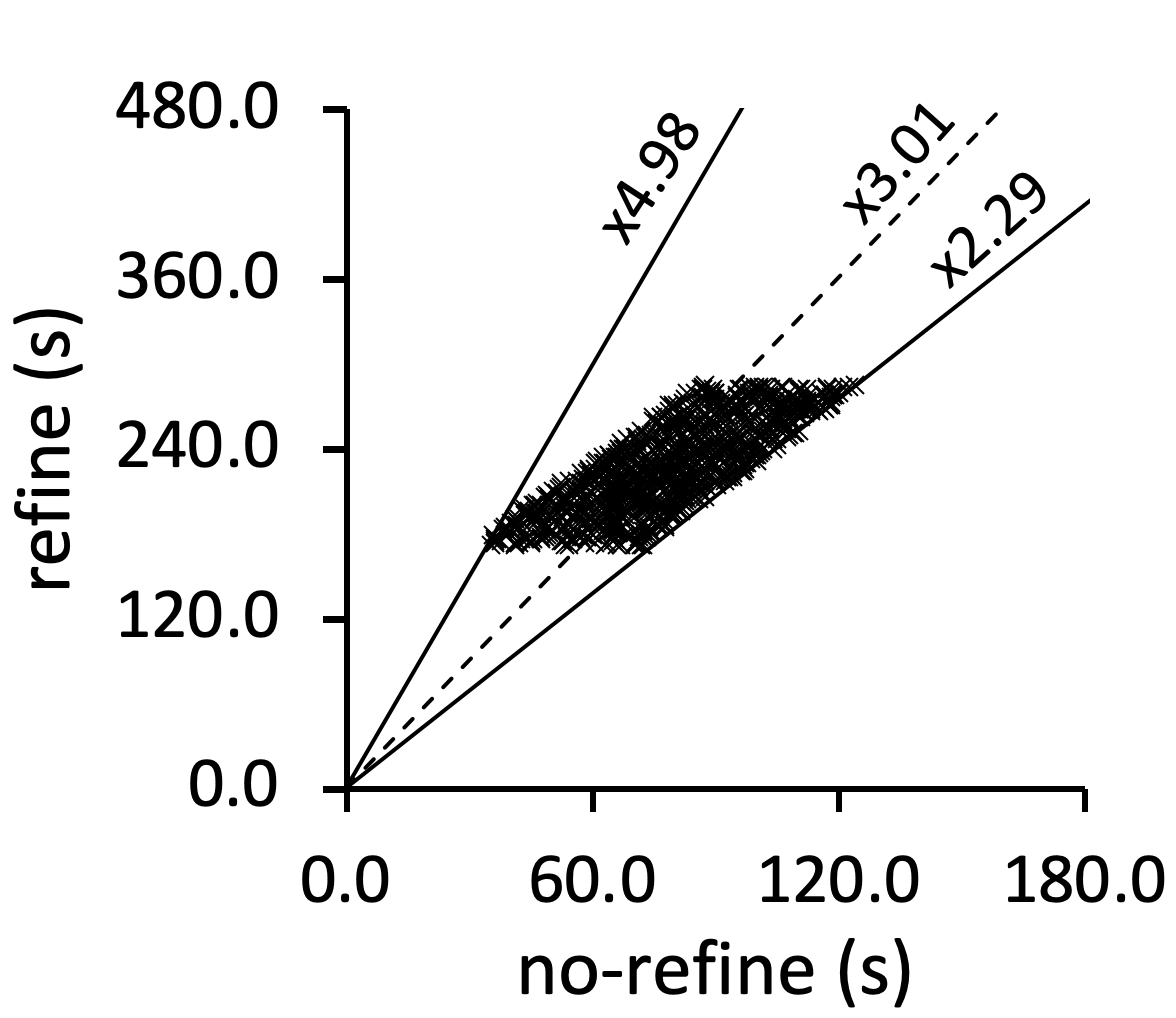
\includegraphics[width=\textwidth]{img/ratio-time}
    \caption{The ratio of time}
  \end{subfigure}
  \caption{Comparison of iterations and analysis time without refinement
  (\stextsf{no-refine}) and with refinement (\stextsf{refine})}
  \label{fig:performance-compare}
  \vspace*{-1.5em}
\end{figure}

\subsection{Effectiveness of Refinement}\label{sec:effect-refine}

\begin{table*}
  \centering
  \caption{Type-related specification bugs newly detected by $\tool$ in the
  official draft of ECMAScript 2021 (ES12)}
  \label{table:new-bug}
  \resizebox{\textwidth}{!}{%
  \begin{tabular}{@{}c@{~}?c|@{~}c@{~}|l|c|@{~}c@{~}|@{~}r@{}}
    \multicolumn{1}{@{}c?}{\textbf{Name}} &
    \multicolumn{1}{c}{\textbf{Feature}} &
    \multicolumn{1}{@{}c@{~}}{\textbf{\#}} &
    \multicolumn{1}{c}{\textbf{Description}} &
    \multicolumn{1}{@{~}c@{~}}{\textbf{Checker}} &
    \multicolumn{1}{@{}c}{\textbf{Created}} &
    \multicolumn{1}{@{}c@{~}}{\textbf{TTL}}\\\specialrule{.1em}{.0em}{.0em}

    ES12-1 &
    Switch &
    3 &
    \makecell[l]{
        Variables \code{hasDuplicates} and \code{hasUndefinedLabels} are already \\
        defined in algorithms for \jscode{case} blocks of \jscode{switch}
        statements.
    } &
    \stextsf{\footnotesize Reference} &
    2015-09-22 &
    1,996 days\\\hline

    ES12-2 &
    Try &
    3 &
    \makecell[l]{
        Variables \code{hasDuplicates} and \code{hasUndefinedLabels} are already \\
        defined in algorithms for \jscode{try} statements.
    } &
    \stextsf{\footnotesize Reference} &
    2015-09-22 &
    1,996 days\\\hline

    ES12-3 &
    Arguments &
    1 &
    \makecell[l]{
        A variable \code{index} is already defined in
        \textbf{CreateMappedArgumentsObject}.
    } &
    \stextsf{\footnotesize Reference} &
    2015-09-22 &
    1,996 days\\\hline

    ES12-4 &
    Array &
    2 &
    \makecell[l]{
        A variable \code{succeeded} is already defined in algorithms for
        \jscode{Array} objects.
    } &
    \stextsf{\footnotesize Reference} &
    2015-09-22 &
    1,996 days\\\hline

    ES12-5 &
    Async &
    1 &
    \makecell[l]{
        A variable \code{value} is already defined in \textbf{Evaluation} for
        \jscode{yield} expressions.
    } &
    \stextsf{\footnotesize Reference} &
    2015-09-22 &
    1,996 days\\\hline

    ES12-6 &
    Class &
    1 &
    \makecell[l]{
        A variable \code{ClassHeritage} is not defined in \textbf{Contains}
        \\ for tails of \jscode{class} declarations.
    } &
    \stextsf{\footnotesize Reference} &
    2015-09-22 &
    1,996 days\\\hline

    ES12-7 &
    Branch &
    1 &
    \makecell[l]{
        A variable \code{Statement} is not defined in \textbf{EarlyErrors} for
        \jscode{if} statement.
    } &
    \stextsf{\footnotesize Reference} &
    2015-09-22 &
    1,996 days\\\hline

    ES12-8 &
    Arguments &
    2 &
    \makecell[l]{
        Abrupt completions are used in \textbf{DefineOwnProperty} and
        \textbf{GetOwnProperty} \\ for \jscode{arguments} objects without any
        checks.
    } &
    \stextsf{\footnotesize Operand} &
    \inred{2015-12-16} &
    \inred{1,910 days}\\
  \end{tabular}
  }
  \vspace*{-1.5em}
\end{table*}

We measured the effectiveness of the condition-based refinement by comparing
the performance and the analysis precision of $\tool$
without (\stextsf{no-refine}) and with refinement (\stextsf{refine}).

For performance comparison, Figure~\ref{fig:performance-compare} presents the
iterations and analysis time without and with refinement.
Figures~\ref{fig:performance-compare}(a) and
\ref{fig:performance-compare}(c) are histograms of the iterations and analysis
time, respectively, and Figures~\ref{fig:performance-compare}(b) and
\ref{fig:performance-compare}(d) are scatter charts for their ratios.
Without refinement, the type analysis took \inred{91.9} seconds with \inred{261.5}K
iterations on average.  For each version, the number of iterations is increased
at least \inred{0.99}x, at most \inred{1.36}x, and \inred{1.16}x on average, and
the analysis time is increased at least \inred{1.05}x, at most \inred{1.99}x,
and \inred{1.41}x on average.

Table~\ref{table:precision} shows the analysis precision without refinement,
with refinement, and their difference.  The refinement improved the analysis
precision from \inred{33.0}\% to \inred{59.2}\% by removing \inred{122}
false-positive bugs and detecting \inred{one} more true bug.  Among six
bug kinds, the most significant improvement is for non-numeric
operand bugs (\stextsf{NoNumber}) from \inred{3.1}\% to \inred{33.3}\%
by removing \inred{59} false-positive bugs.  The refinement technique
successfully prunes out non-numeric values for numeric types.
The refinement also significantly increased the analysis precision for unknown
variable bugs (\stextsf{UnknownVar}) and assertion failures
(\stextsf{Assertion}) by removing \inred{29} and \inred{25} false-positive bugs, respectively.
Because $\tool$ can precisely analyze callees of function invocations
without refinement, we found no improvement for missing
parameter bugs (\stextsf{MissingParam}).


\subsection{Detection of New Bugs}\label{sec:new-bug}

Among \inred{93} true bugs detected by $\tool$, \inred{14} are newly
detected and still exist in the latest version of ECMAScript.
Table~\ref{table:new-bug} summarizes the bugs, their
related JavaScript language features, and their TTLs.
Except for two bugs in ES12-8, all bugs were introduced in the initial
commit of the open development on September 22, 2015.
Thus, 12 newly detected bugs last for 1,966 days until March 9, 2021.
The two bugs in ES12-8 were created when a contributor introduced
the prefixes \textbf{?} and \textbf{!} on December 16, 2015, and they last for 1,910 days.
We reported the newly detected bugs to TC39, and all of them were
confirmed by the committee and will be fixed in ECMAScript 2022 (ES13).

ES12-1 contains three bugs due to duplicated variable declarations
in three syntax-directed algorithms for the \jscode{case} block
of the \jscode{switch} statement:
\code{hasDuplicates} in \textbf{ContainsDuplicateLabels} and
\code{hasUndefinedLabels} in \textbf{ContainsUndefinedBreakTarget} and
\textbf{ContainsUndefinedContinueTarget}.
A \jscode{case} block optionally contains \jscode{case} clauses.
In the beginning of three algorithms,
\code{hasDuplicates} or \code{hasUndefinedLabels} is defined if the clauses exist.
However, because the same variable is defined again after the conditional steps,
three algorithms for \jscode{case} blocks
with \jscode{case} clauses always have the duplicated variable declaration bugs for
\code{hasDuplicates} or \code{hasUndefinedLabels}.
Similarly, ES12-2 contains three bugs caused by the same reason in the
same abstract algorithms for the \jscode{try} statement.

The bug in ES12-3 is a reference bug for a duplicated declaration of the variable
\code{index} in the abstract algorithm \textbf{CreateMappedArgumentsObject}.
For each function call in JavaScript programs, an \jscode{arguments} object is
created by \textbf{CreateMappedArgumentsObject}.  In the algorithm, the variable
\code{index} is defined to handle the index of a given list of arguments.
However, the variable is defined twice in step 14 and 17 of the algorithm.

ES12-4 contains two reference bugs for the already defined variable \code{succeeded}
in \textbf{DefineOwnProperty} of \jscode{Array} objects and
\textbf{ArraySetLength}.  The \jscode{Array} objects are
not ordinary objects and have special algorithms for specific behaviors.
Two such algorithms are wrapper algorithms of
\textbf{OrdinaryDefineOwnProperty}, which updates object properties.
While they define the variable \code{succeeded} to represent the result of
\textbf{OrdinaryDefineOwnProperty}, the variable is defined twice in a specific condition.

The bug in ES12-5 is a reference bug for the already defined variable \code{value}
in \textbf{Evaluation} of the \jscode{yield *} expression.
  In the evaluation of \jscode{yield * e}, the variable \code{value} is defined twice to
represent 1) the evaluation result of the given expression \jscode{e} in step
3, and 2) the iterator value in step 7.c.viii.1.

The bug in ES12-6 is a reference bug for the unknown variable \code{ClassHeritage}
in \textbf{Contains} for the tails of \jscode{class} declarations.  A tail of a
\jscode{class} declaration consists of an optional class extension with the
\jscode{extends} keyword and a class body.  When the
optional class extension does not exist, the variable \code{ClassHeritage} is not
defined but the \textbf{Contains} algorithm tries to access it without any check
of its existence.

The bug in ES12-7 is a reference bug for the unknown variable \code{Statement} in
\textbf{EarlyErrors} for the \jscode{if} statement.  In syntax-directed algorithms,
when a production produces multiple sub-ASTs, it uses ordinal numbers as prefixes of variables.
Because the \jscode{if} statement contains two sub-ASTs
produced by the \textit{Statement} production, the ordinal number prefixes
are necessary for the variable \code{Statement}.  However, the
\textbf{EarlyErrors} algorithm for the \jscode{if} statement uses the variable without any
ordinal number prefixes.

ES12-8 contains two operand type bugs related to abrupt completions in
\textbf{DefineOwnProperty} and \textbf{GetOwnProperty} for \jscode{arguments} objects.
The two algorithms define or get own properties of \jscode{arguments} objects.
They use the \textbf{Get} algorithm, which returns JavaScript
values stored in object properties or abrupt completions.
Thus, they should check whether the results of \textbf{Get} are abstract completions or not
before using them but they use the results without any checking of abrupt completion.
